\documentclass[../../Instructions_Framework]{subfiles}
% Hier müssen keine Packages geladen werden, es werden automatisch die von masterdoc geladen,
% sowie die Konfigurationen.
% Bei includegraphics nur Bildname (Bsp: Bild.png) eingeben, da er in den angegebenen Pfade die Bilder sucht
\graphicspath{{img/}{img/}}

\begin{document}

\chapter{Instructions for creating an interaction technique}
\label{technique}

This chapter explains how to implement your own interaction technique using our framework. For creating your own technique please refer to the following instructions. Choose the technique you want to use.

\section{Technique}
\begin{enumerate}
	\item Go in the project structur to \textbf{Assets/BullsEye/Examples/Scripts} and create by right click a new C\# script. The name is up to you.
	\begin{itemize}
		\item \textbf{Object interaction}: Attach the newly created script to the object which you want to interact with.
		\item \textbf{Not object related}: If you want to create an interaction technique which is not object related, you should create a new empty game object and attach the script at it.
	\end{itemize}
	\item This new script has to extend the \textit{MonoBehaviour} class provided by unity and additionally implement one of the interfaces from our framework depending on which kind of interaction technique you want to create. Click in the inspector area on the right hand side at addComponent and search for your script by entering the name you choose. For open the script click on the right hand side at the gear. For import the interface methods click on "Import the missing members", select all and finish (for fixation look at Fig. \ref{vs}). When you use Visual Studio you need to delete the exceptions in the genereated classes (see in Fig. \ref{delete}).
	\newpage
	
	\begin{figure}[htb]
		\centering
		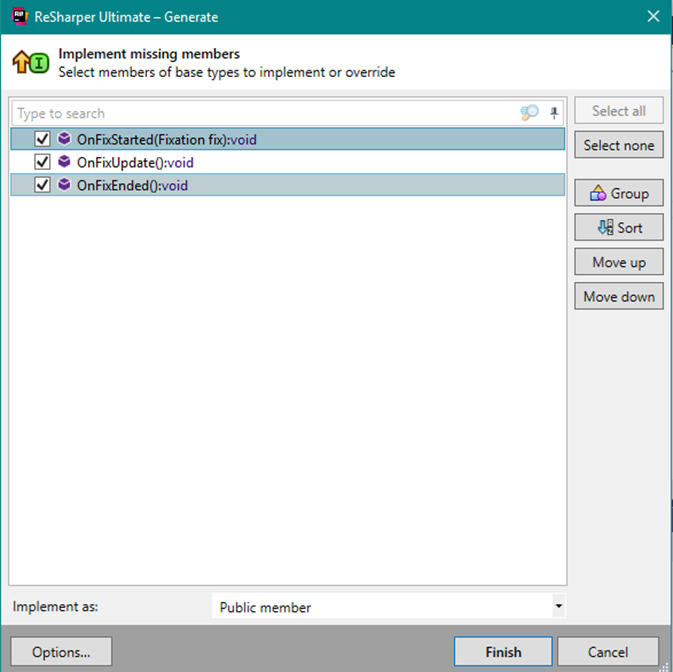
\includegraphics[width=0.5\linewidth]{img/screenshot001}
		\caption{Missing imports}
		\label{vs}
	\end{figure}
	\begin{figure}[htb]
		\centering
		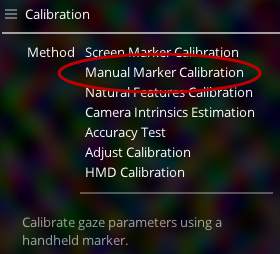
\includegraphics[width=0.5\linewidth]{img/screenshot006}
		\caption{Exceptions}
		\label{delete}
	\end{figure}
	

\end{enumerate}
\subsection{Fixation technique}
\begin{itemize}
	\item If you want to create a fixation interaction technique, you'll have to implement the \textit{IFixationInteractionTechnique} interface (see in Fig. \ref{classHeader}).\\
	\begin{figure}
		\centering
		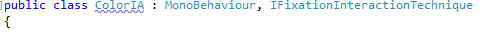
\includegraphics[width=0.7\linewidth]{img/InterfaceFix}
		\caption{Class header after extending \textit{MonoBehaviour} and implementing the \textit{IFixationInteractionTechnique} interface}
		\label{classHeader}
	\end{figure}
	This interface defines three methods:
	\begin{itemize}
		\item \textit{OnFixStarted} which is called at the start of a new fixation and provides a \textit{Fixation} object which contains information about the fixation, like the position on the screen.
		\item \textit{OnFixUpdate} which is called every frame like the Update method provided by Unity, but just while the fixation is still ongoing.
		\item \textit{OnFixEnded} which is called once the fixation ends.
	\end{itemize}

\end{itemize}
\subsection{Gesture technique}
\begin{itemize}
\item If you want to create a gesture interaction technique, you'll have to implement the \textit{IGestureInteractionTechnique} interface (see in Fig. \ref{fig:interfacegesten}).
\item Additionally you have to create a gesture which triggers the technique. Creating the gesture is using simplest the external tool \textit{GestureCreator} (see in Fig \ref{fig:creator}) which generates the constructor for the entered gesture which you can easily copy to the \textit{Start} method before the \textit{Subscribe} method is called. You can find it in the Unity editor  in the Assets/Editor folder.\\

\begin{figure}
	\centering
	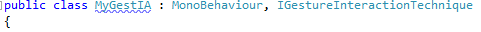
\includegraphics[width=0.7\linewidth]{img/InterfaceGest}
	\caption{Class header after extending \textit{MonoBehaviour} and implementing the \textit{IGestureInteractionTechnique} interface}
	\label{fig:interfacegesten}
\end{figure}
\begin{figure}
	\centering
	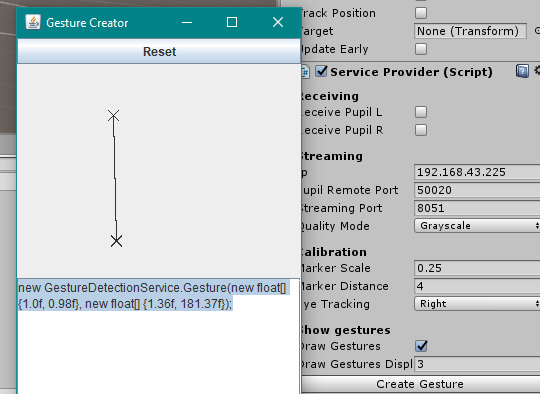
\includegraphics[width=0.7\linewidth]{img/creator}
	\caption{Gesture creator}
	\label{fig:creator}
\end{figure}
This interface provides only the method \textit{OnGesture} which is called every time the defined gesture is entered via fixations and saccades.
\end{itemize}
\subsection{Pursuit technique}
\begin{figure}
	\centering
	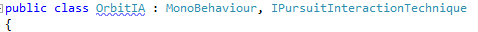
\includegraphics[width=0.7\linewidth]{img/InterfacePur}
	\caption{Class header after extending \textit{MonoBehaviour} and implementing the \textit{IPursuitInteractionTechnique} interface}
	\label{fig:interfacepur}
\end{figure}
\begin{itemize}
	\item If you want to create a pursuit interaction technique, you'll have to implement the \textit{IPursuitInteractionTechnique} interface (see in Fig. \ref{fig:interfacepur}).\\
	This Interface defines two methods, you have to implement:
	\begin{itemize}
		\item \textit{OnPursuitUpdate} which is called every frame like the Update method provided by Unity. Via the parameter object you can get information about the current state of the pursuit.
		\item \textit{OnPursuit} which is called as soon as the conditions from the subscribtion are met.
	\end{itemize}
\end{itemize}


\subsection{Service Provider}
\begin{itemize}	
	\item Now call the \textit{ServiceProvider.Get} method in the \textit{Start} method inherited from the \textit{MonoBehaviour} class and use either \textit{FixationDetectionService}, \textit{GestureDetectionService}, or \textit{PursuitDetectionService} as the generic type. Figure \ref{fig:startpur} shows a \textit{Start} method in which an interaction technique subscribes itself to the \textit{PursuitDetectionService}.\\ The services accept different parameters for their subscription methods with them you can further specify your wished behaviour.\\
	\item The \textit{FixationDetectionService} needs a reference to the script itself as its only mandatory parameter. Furthermore there are optional parameters with them you can specify whether you want the interaction technique only triggers if the \textit{GameObject} the script is attached to is the target of the fixation, default option for this parameter is \textit{true}.\\
	As next parameter you can enter an array of to \textit{Vector2} objects to declare an area on the screen and only if the fixation is within this area or set it to \textit{null} in which case this condition isn't checked. No given array is the default option.\\
	The next parameter is the time in milliseconds for which all eye tracking data is checked for a possible fixation. The default parameter is 200 because it is the minimal time needed for the human brain to fixate an object.\\
	The latest parameter is the permitted deviation of gaze points during the prior defined time span in pixels. Higher values in this parameter cause more scattered gaze points to still trigger the interaction technique. The default value is 100 because our test showed that this value results in the most reliable detection of fixations (see in Fig. \ref{fig:startfix}).
	\begin{figure}[h!]
		\centering
		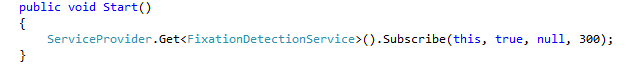
\includegraphics[width=0.7\linewidth]{img/StartFix}
		\caption{Start method FixationDetectionService}
		\label{fig:startfix}
	\end{figure}
	\item The \textit{GestureDetectionService} requires not only the reference to the script itself, but also the created gesture as parameters. The first optional parameter is the allowed deviation for angles between the angle specified in the gesture's constructor and the entered angle via eye tracking data. It is given as percentage of 360 degrees. The default parameter is 0.05 which equals a deviation of up to 18 degrees to either side.\\
	The other optional parameter is the allowed deviation in length between defined and entered edges. It is given as percentage. The default parameter is 0.1 which results in edges having between 90\% and 110\% of the defined length are permitted (see in Fig. \ref{startGesture}).
	\begin{figure}[h!]
		\centering
		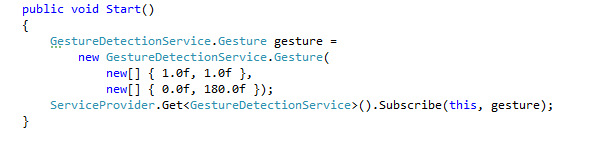
\includegraphics[width=0.7\linewidth]{img/StartGest}
		\caption{Start method GestureDetectionService}
		\label{startGesture}
	\end{figure}
	\item The \textit{PursuitDetectionService} also requires a reference to the script itself as its first parameter. The second mandatory parameter is the time the object has to be followed for the interaction to trigger. The last parameter is the correlation threshold. This threshold must be met before the interaction can be triggered, the default value is 0.9 (see in Fig. \ref{fig:startpur})
	\begin{figure}[h!]
		\centering
		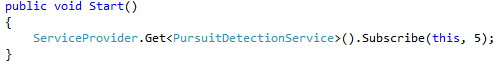
\includegraphics[width=0.7\linewidth]{img/StartPur}
		\caption{Start method PursuitDetectionService}
		\label{fig:startpur}
	\end{figure}
	\end{itemize}

\end{document}